\chapter{Description of [APPNAME]}
\label{chp:description}

This chapter will give a description of [APPNAME], through textual description and screen shots.

\section{Basic System Architecture}
Figure \ref{fig:basic-architecture} shows an overview of the architecture we intend to use for our solution. We will build upon the architecture used by Aaberg et. al. \cite{CustomerDriven}.

We have access to a MySQL-server hosted at NTNU, which we will access by a PHP-server hosted at NTNU. The main reason we have to access the database through a server layer, is that it is quite cumbersome to connect to the database if a device is not connected at NTNU's network. In addition, by having a webservice do some of the work for us, it becomes easier to parse results from the database through JSON.   


The downside by having this approach is that scalability suffers from this architectural choice. However, we consider these problems as outside the scope of our thesis, and will continue using this approach.

\begin{figure}
		\centering
			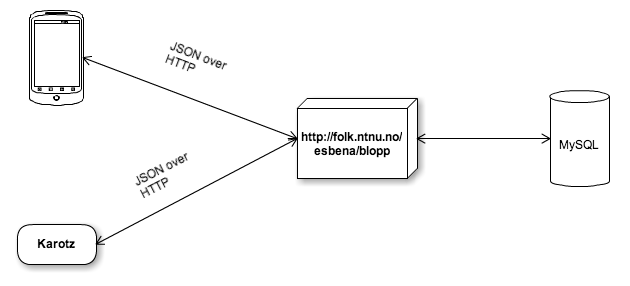
\includegraphics[width=0.50\paperwidth]{Pictures/basic-architecture.png}
		\caption{Basic architecture of our system}
		\label{fig:basic-architecture}
\end{figure}

\section{Child partition}
The child partition of our application consists mainly out of four parts. When Aaberg et. al. created the original application, they wanted a conceptual look and feel throughout the applications. They used images of Karotz in the application in order to introduce a sense of completeness, i.e. the Karotz bound CAPP, GAPP and KAPP together. [TODO: Vi burde bytte ut Karotz-bilder med eget produkt imo]. 

\paragraph{Treatment}
Figure \ref{fig:capp_start_treatment} shows a screenshot for the application when the child starts their medication. Starting this sequence can come from one out of two events: (i) \emph{The child reacts to an alarm set in the guardian partition}, and (ii) \emph{The child needs to take their medicine by need}. If (ii) is the case, the child is instructed to pick the medicine from a list shown by the application. If (i) is the case, the medicine is chosen beforehand. When a child has started their treatment, they are taken through an animated sequence, which reacts when a child interacts with the device.  



\paragraph{Showing rewards}

Figure \ref{fig:capp_stars} shows a screenshot for the application when the child wants to review how many stars he/she has received, based on the amount of medicine they have taken. We have made two design decisions for our reward system. First, we never want stars to be removed. We don\'t want children to feel that credits are being removed from them. Second, we can\'t assume children are able to read, and thus we have made it countable, and hopefully they can comprehend how many stars they've actually got. In addition, we provide some help to those who are able to read numbers, by showing the amount of stars a child has on the top. The downside here comes when a child has been given like 200 treatments. This will obscure the view a bit.     

\paragraph{Shop}
In the shop, children are allowed to buy rewards from parents [Insert Reference]. Figure \ref{fig:capp_store} shows a inside-view of our shop. Children can buy an activity by pressing the selected activity. Due to time constraints, we have not been able to implement voice over, so the children will have to find a parent who can read it if they are not able to [TODO: 1: Bryter med linjen over. 2: Implementasjon av voice over med norsk som språk er vanskelig]. 



\paragraph{Treatment instructions}
The treatment instructions is a book-styled instruction set which shows generically how to take a medicine. 
The following steps are included in instructions: 
\begin{enumerate}
  \item Shake the inhaler such that the particles loosen up. 
  \item Take the cap of the inhaler
  \item Attach the inhaler to the inhaling chamber [TODO: Korrekt bruk?]
  \item Put the inhaler onto the face of the child
  \item Press the inhaler until you hear a sound
  \item Let the child breathe calmly 10 times in and out
  \item Let the child wash his/her mouth
\end{enumerate} 



\begin{figure}
	\begin{minipage}[b]{0.4\linewidth}
		\centering
			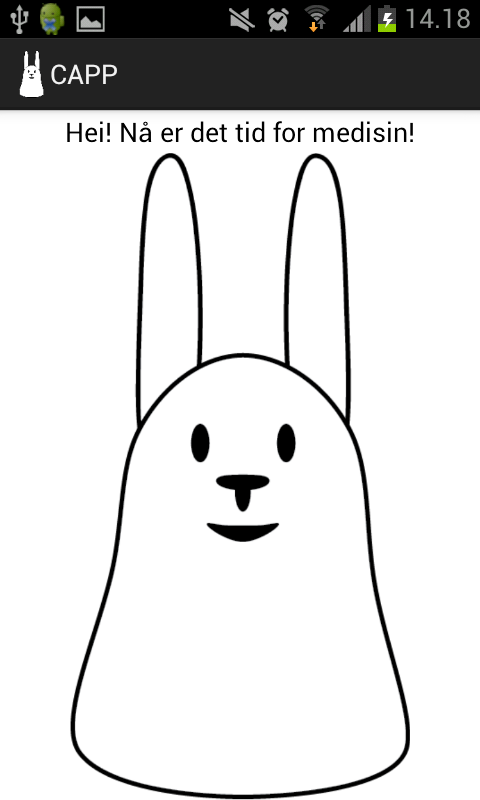
\includegraphics[width=0.20\paperwidth]{Pictures/app-screenshots/capp_start_treatment.png}
		\caption{Starting a treatment}
		\label{fig:capp_start_treatment}
	\end{minipage}
	\hspace{3cm}
	\begin{minipage}[b]{0.4\linewidth}
		\centering
			
\includegraphics[width=0.20\paperwidth]{Pictures/app-screenshots/capp_stars.png}
		\caption{SHOULD BE A SHOP}
		\label{fig:capp_store}
	\end{minipage} 
\end{figure}

\begin{figure}
	\begin{minipage}[b]{0.4\linewidth}
		\centering
		
\includegraphics[width=0.20\paperwidth]{Pictures/app-screenshots/capp_stars.png}
		\caption{Rewards}
		\label{fig:capp_stars}
	\end{minipage}
	\hspace{3cm}
	\begin{minipage}[b]{0.4\linewidth}
		\centering
		
\includegraphics[width=0.20\paperwidth]{Pictures/app-screenshots/capp_stars.png}
		\caption{SHOULD BE A MANUAL}
		\label{fig:change_me}
	\end{minipage}
\end{figure}

\section{Guardian partition}
Dette er en mergesolve.



% Skjermbilder -> Forklaringer
% Dropper alt som har med Karotz å gjøre, med unntak av ``konsept''-følelsen
% 